\documentclass{article}
\usepackage{hyperref}
\usepackage{float}
\usepackage[margin=1in]{geometry}
\usepackage[justification=centering]{caption}
\usepackage{amsmath,amsfonts,amsthm,fullpage,amssymb,algorithm,color,mathtools,float,hyperref,subcaption,url,graphicx, algorithmic}
\usepackage[document]{ragged2e}
\newcommand{\largeimagewidth}{350}
\newcommand{\mediumimagewidth}{250}
\setlength{\parskip}{1em}
\begin{document}
\begin{titlepage}
\clearpage\thispagestyle{empty}
\centering
\vspace{1cm}

\rule{\linewidth}{1mm} \\[0.5cm]
{ \Large \bfseries ISYE 6740 - Fall 2023\\[0.2cm]
Final Project}\\[0.5cm]
\rule{\linewidth}{1mm} \\[1cm]

\begin{tabular}{l p{5cm}}
\textbf{Team Member Names:} William Luna (Solo) gtID: 903947280 &   \\[10pt]
\textbf{Project Title:} Speaker Attribution in Written Dialogue &  \\[10pt]
\end{tabular} 

\tableofcontents
\newpage

\section{Problem Statement}

\justifying{Effective dialogue in storytelling requires that each character speak distinctly. The purpose of having multiple characters in a story is to provide a diversity of opinions, perspectives, and backgrounds. If every sentence spoken feels appropriate coming out of the mouth of any character, why have multiple characters at all? How bland would the adventures of Harry, Ron, and Hermione be if all three were equal parts courageous, loyal, and inquisitive, instead of each personality compensating for the other two? Would \textit{Pride and Prejudice} be effective at exposing class inequalities in Victorian society if every character sounded equally posh?}

\justifying{However, empirically evaluating the distinctness of each character's dialogue in a story is a subjective and challenging process.}

\justifying{This project proposes a methodology to evaluate the distinctness between sets of dialogue in terms of vocabulary and style. Then, through applying this methodology to dialogue in television shows and films, assesses the ability to predict either a) the speaker within a piece of media, where the corpus is a single piece of media, or b) from which piece of media a line of dialogue originated, where the corpus spans several pieces of media . This distinction will be referred to as $Within-Media$ and $Across-Media$ Classifications going forward.}

\justifying{We will conclude with a discussion of the success of the models at speaker/media classification, how they may be applied to evaluate whether character dialogue has a sufficiently unique voice, and areas of future exploration.}

\section{Data Collection}

The corpus for this project was curated from several data sources that provide dialogue from popular movies, television shows, and books:

- \href{https://www.kaggle.com/datasets/blessondensil294/friends-tv-series-screenplay-script/data?select=S01E01+Monica+Gets+A+Roommate.txt}{Friends}: kaggle.com/datasets/blessondensil294/friends-tv-series-screenplay-script/
 
- \href{https://www.kaggle.com/datasets/pierremegret/dialogue-lines-of-the-simpsons}{The Simpsons}: kaggle.com/datasets/pierremegret/dialogue-lines-of-the-simpsons

- \href{https://www.kaggle.com/datasets/paultimothymooney/lord-of-the-rings-data?select=lotr_scripts.csv}{The Lord of the Rings}: kaggle.com/datasets/paultimothymooney/lord-of-the-rings-data

- \href{https://www.kaggle.com/datasets/andradaolteanu/rickmorty-scripts}{Rick and Morty}: kaggle.com/datasets/andradaolteanu/rickmorty-scripts

- \href{https://scriptline.livejournal.com/71215.html#cutid6}{Pride and Prejudice, Downtown Abbey*}: scriptline.livejournal.com/71215.html

After data cleaning, the outcome is a corpus of the following format. In order to make visualizations easier to interpret, and remove characters with too little data, the dialogue from only the six most frequently occurring characters from each media are used:

\begin{table}[H]
    \centering
    \begin{tabular}{|c|c|c|}
        \hline
        \textbf{} \textbf{media} & \textbf{speaker} & \textbf{dialogue} \\
        \hline
        Friends & Phoebe &  ``I asked for the news, not the weather.'' \\
        Friends & Phoebe &  ``You'll see. You'll all see.'' \\
        Friends & Joey &  ``How you doin'?'' \\
        Pride and Prejudice & Mr. Darcy &  ``My affections and wishes have not changed, but...''  \\
        The Lord of the Rings & Gandalf &  ``Fly you fools!'' \\
        \hline
    \end{tabular}
    \caption{Sample Rows from Dialogue Speaker Corpus}
    \label{tab:images}
\end{table}

\section{Methodology}
\subsection{Feature Engineering}
\subsubsection{Heuristics}
There are multiple frameworks for evaluating the uniqueness between two sets of text. Two were chosen to serve as heuristics for this research–Yule's K and Simpson's D.

\textbf{Yule's K} is a calculation that estimates the variety of vocabulary in a text^1:

Given:

- $N$ as the total number of words in a text

- $V(N)$ as the number of distinct words

- $V(m, N)$ as the number of words appearing m times in the text

- ${m_{\text{max}}}$ as the largest frequency of a word,

it is defined as:

\[
S_1 = \sum_{m} mV(m, N), S_2 = \sum_{m} m^2V(m, N)
\]

\[
K = C^2 \frac{S_2 - S_1}{S_1^2} = C \left[ - \frac{1}{N} + \sum_{m=1}^{m_{\text{max}}} V(m, N) \left( \frac{m}{N} \right)^2 \right]
\]

\textbf{Simpson's D} (formally Simpson's Diversity Index) was created as a measure of diversity within an ecological community^2. 

However, it can also be applied as a measure of variety in a text corpus. Given:

- $n$ as a vector that represents all the distinct words in the corpus

- $i$ as a particular word in the corpus

- $n_i$ as the number of times word $i$ occurs in the corpus

- $N$ as the total number of words in the corpus

it is defined as:

\[
D = \frac{\sum_{i=1}^{n} n_i(n_i - 1)}{N(N - 1)}
\]

Treating the dialogue of each speaker as its own corpus, we calculate Yule's K and Simpson's D for each, plotting the variation:

\begin{figure}[H]
\centering
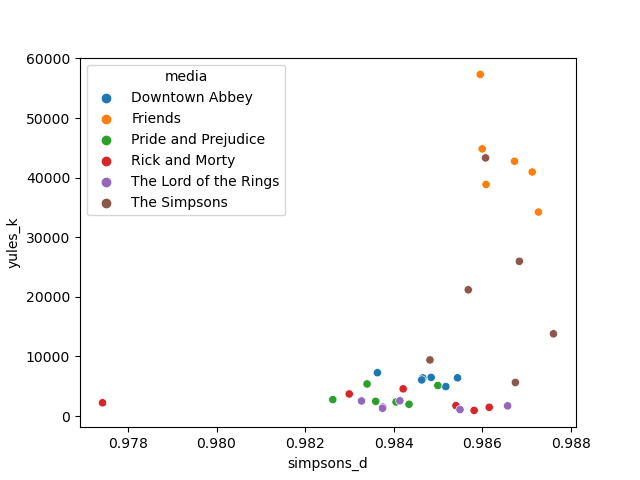
\includegraphics[width=\largeimagewidth]{images/heuristics.png}
\caption{Yule's K, a heuristic created specifically to measure text, exposes more variability in dialogue.}
\end{figure}

Despite Yule's K's separation of characters in \textit{The Simpsons} and \textit{Friends} compared to the other media, it does not appear likely that these heuristics would be sufficient classifying from which piece of media a speaker originated.

However, when comparing speakers within the same media, simple patterns can emerge. In the charts below, characters co-locate on the scatter plot based on their function in the story. Frodo and Sam spend much of \textit{The Lord of the Rings} traveling together, as do Merry and Pippin. Rick and Morty are the protagonists of the eponymous show, while Beth, Jerry, and Summer are the supporting cast:

\begin{figure}[H]
    \centering
    \caption{Selected Within-Media Plots}
    \begin{subfigure}[b]{0.45\textwidth}
        \centering
        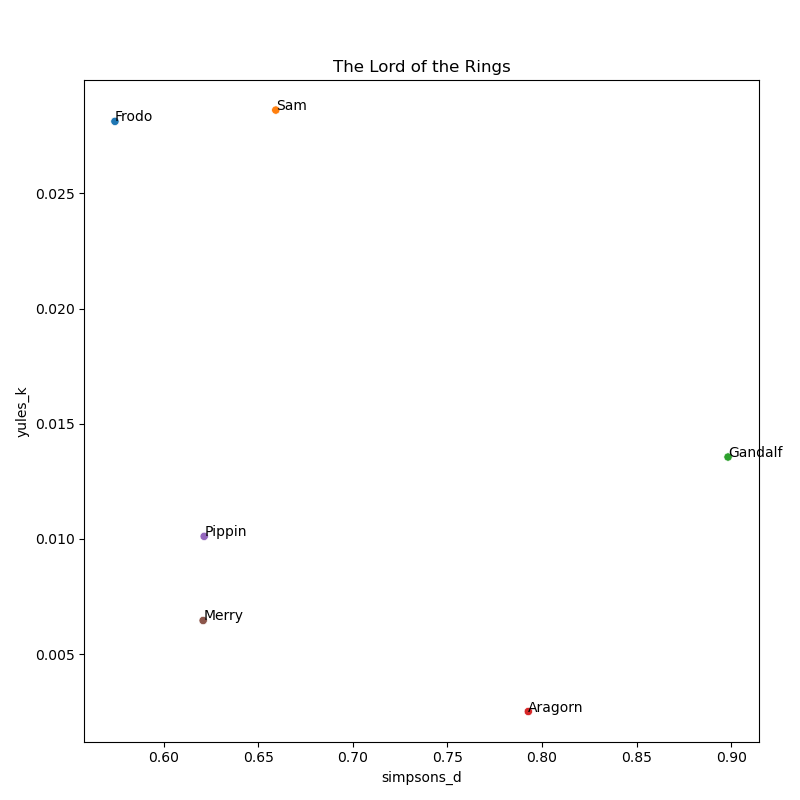
\includegraphics[width=\textwidth]{images/The Lord of the Rings_heuristics.png}
        \caption{The Lord of the Rings}
        \label{fig:subfig1}
    \end{subfigure}
    \hfill
    \begin{subfigure}[b]{0.45\textwidth}
        \centering
        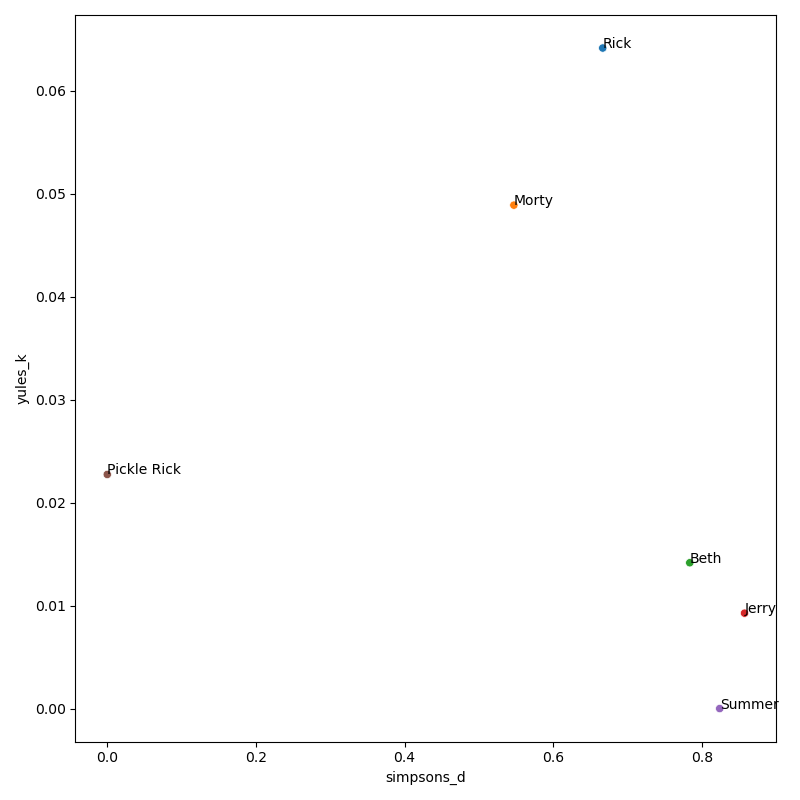
\includegraphics[width=\textwidth]{images/Rick and Morty_heuristics.png}
        \caption{Rick and Morty}
        \label{fig:subfig2}
    \end{subfigure}
    \label{fig:main}
\end{figure} 

One important takeaway from this heuristic analysis is that for the media in the corpus, the differences in dialogue \textit{across} each media (TV show, film, book) are greater than the differences of dialogue between each character \textit{within} the same piece of media.

\subsubsection{Stylometry}

While Stylometry's technical definition is ``the statistical analysis of variations in literary style,'' for this section, it is better explained by Augustus de Morgen's original 1851 definition of ``if one text `deals in longer words' than another''^3.

To prepare the data for this section, all dialogue for each speaker was converted into frequency distributions of sentence and word length. In other words, how many words did a speaker use in each sentence, and how many characters did they use in each word?

\textit{The Lord of the Rings} is shown here as an illustrative example of all the within-media plots. Most look similar, where despite the fact that one speaker may have a unique distribution (Gandalf below), the majority of the characters' distributions are extremely similar.

However, as we see in the chart on the right, the variance of the distributions are greater across-media:

\begin{figure}[H]
    \centering
    \caption{Within- and Across- Media Sentence Length Distributions}
    \begin{subfigure}[b]{0.45\textwidth}
        \centering
        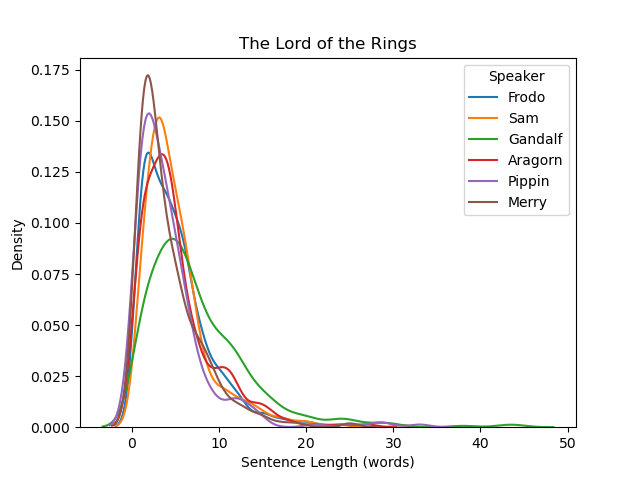
\includegraphics[width=\textwidth]{images/The Lord of the Rings_sentence_length.png}
        \caption{The Lord of the Rings}
        \label{fig:subfig1}
    \end{subfigure}
    \hfill
    \begin{subfigure}[b]{0.45\textwidth}
        \centering
        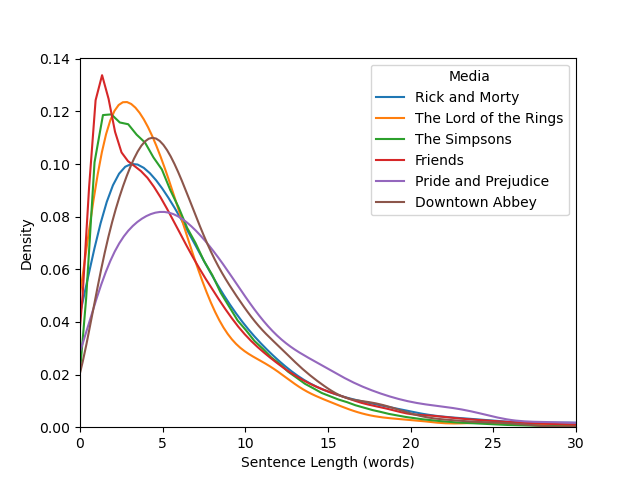
\includegraphics[width=\textwidth]{images/overall_sentence_length.png}
        \caption{Overall}
        \label{fig:subfig2}
    \end{subfigure}
    \label{fig:main}
\end{figure} 

Plotting both within- and across-media Kernel Density Estimators (KDEs) $f(x) = \frac{1}{nh} \sum_{i=1}^{n} K\left(\frac{x - x_i}{h}\right)$,
it is unclear whether the variation in sentence and word length is sufficient to provide predictive features to a classifier:

\begin{figure}[H]
    \centering
    \caption{Selected KDE Plots}
    \begin{subfigure}[b]{0.45\textwidth}
        \centering
        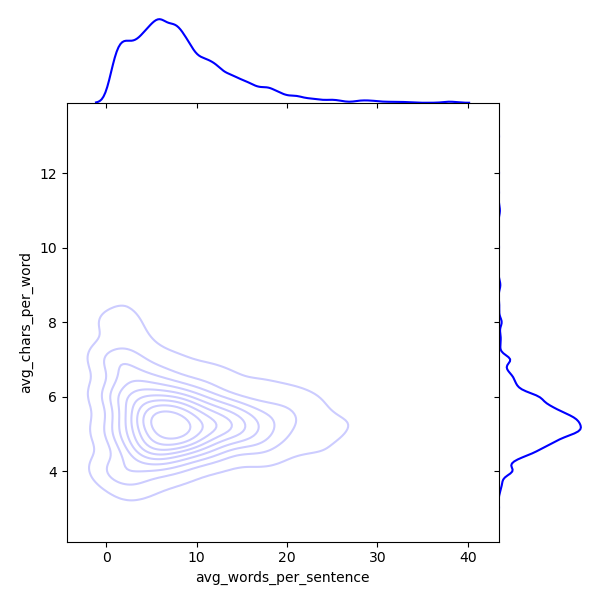
\includegraphics[width=\textwidth]{images/3d_kde_test_0.png}
        \caption{Pride and Prejudice}
        \label{fig:subfig1}
    \end{subfigure}
    \hfill
    \begin{subfigure}[b]{0.45\textwidth}
        \centering
        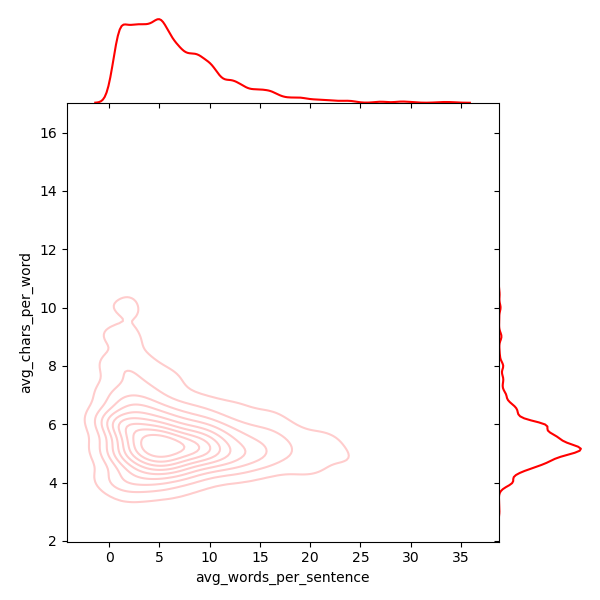
\includegraphics[width=\textwidth]{images/3d_kde_test_1.png}
        \caption{Friends}
        \label{fig:subfig2}
    \end{subfigure}
    \label{fig:main}
\end{figure} 

\begin{figure}[H]
\centering
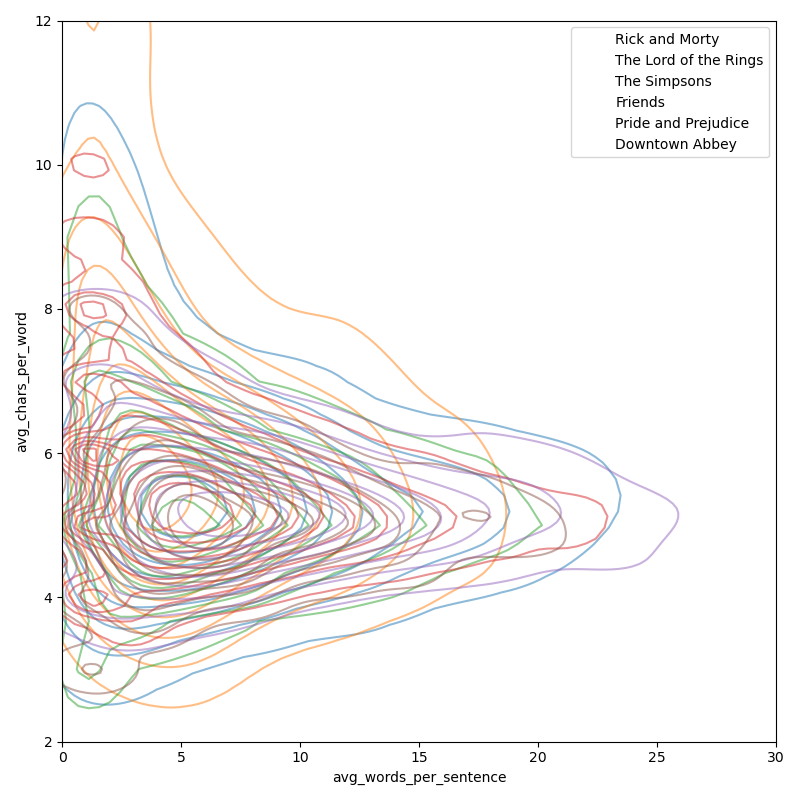
\includegraphics[width=\largeimagewidth]{images/3d_kde_test_final.png}
\caption{Across-media KDE Plots. Media with more sophisticated dialogue (\textit{Pride and Prejudice}, \textit{Downtown Abbey}) have wider word- and sentence-length distributions than American Sitcoms (\textit{The Simpsons}, \textit{Friends}).}
\end{figure}

To assess the potential value of incorporating stylometry into a classifier model, A KDE classifier was created to predict in which media a given line of dialogue was spoken. Given that the accuracy of the model was near-random (approx. 15 percent), and the evidence that dialogue variation is greater across media than within media, I concluded that stylometry, at least at this level of rudimentary implementation, was unlikely to contribute to an effective classifier.

\subsubsection{Vocabulary}

Vocabulary is more commonly used to train text classifiers than stylometry or the heuristics explored above. In Natural Language Processing, a common way of creating features from text vocabulary is \textbf{Term Frequency-Inverse Document Frequency}.

My own simple, imprecise definition is: ``how much more or less does this word occur in this text sample compared to how often it occurs in a larger corpora?''

Where the precise definition follows:
\[
\text{TF}(t, d) = \frac{\text{Number of times term } t \text{ appears in a document } d}{\text{Total number of terms in the document}}
\]
\[
\text{IDF}(t, D) = \log \left( \frac{\text{Number of documents}}{\text{Number of documents containing term } t} \right)
\]
\[
\text{TF-IDF}(t, d, D) = \text{TF}(t, d) \times \text{IDF}(t, D)
\]

It's important to note that the definition of a ``document'' depends on whether an Across- or Within- Media analysis is being performed. For Across-Media, the full corpus of each show or film represents a document, where for Within-Media, all the dialogue for a specific speaker represents a document. In both cases, the result of performing TF-IDF is a matrix of dimensions $NxM$, where $N$ is the number of documents and $M$ is the number of terms in a document. Since many media have vocabulary that is not used in any other piece of media, we should expect the result to be a sparse matrix.

Before training a classifier, K-means Clustering was performed on the top two principal components of the TF-IDF matrix, to create a scatter plot that provides a visual intuition for the efficacy of this method. The resulting low mis-classification rate indicates that vocabulary provides more effective predictor variables than those explored earlier:

\begin{figure}[H]
    \centering
    \caption{PCA Assessment of TF-IDF}
    \begin{subfigure}[b]{0.45\textwidth}
        \centering
        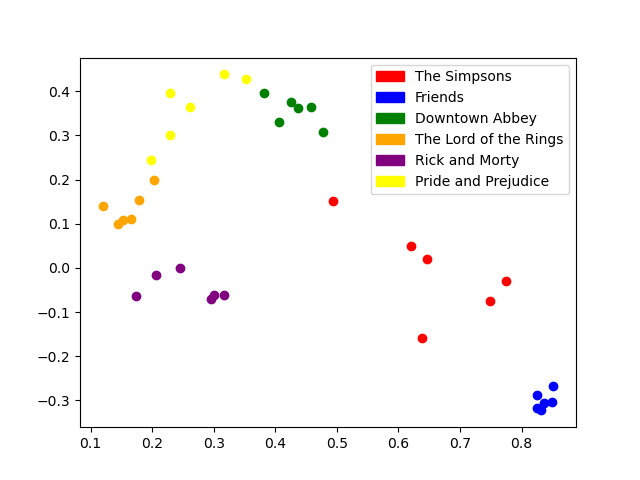
\includegraphics[width=\textwidth]{images/k_means_across_media_misclassifications.png}
        \caption{Actual Labels}
        \label{fig:subfig1}
    \end{subfigure}
    \hfill
    \begin{subfigure}[b]{0.45\textwidth}
        \centering
        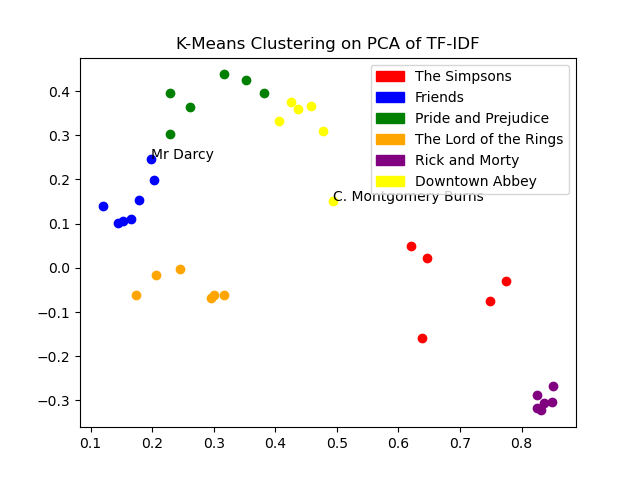
\includegraphics[width=\textwidth]{images/k_means_across_media_predicted.png}
        \caption{K Means Clustering (misclassifications in bold)}
        \label{fig:subfig2}
    \end{subfigure}
    \label{fig:main}
\end{figure} 

Some hypotheses about the misclassifications highlighted on the right:

1. Wealthy power plant owner Mr. Burns is misclassified as being in \textit{Downtown Abbey} (instead of \textit{The Simpsons}), a show that depicts elite society in Victorian England.

2. Aristocratic (and arrogant) Mr. Darcy is misclassified as being in \textit{The Lord of the Rings} (instead of \textit{Pride and Prejudice}) for having a similar vocabulary to the wizard Gandalf.

3. Mr. Carson is misclassified as being part of \textit{Pride and Prejudice} (instead of \textit{Downtown Abbey}), for presumably speaking more formally by virtue of being the head butler.

\begin{figure}[H]
\centering
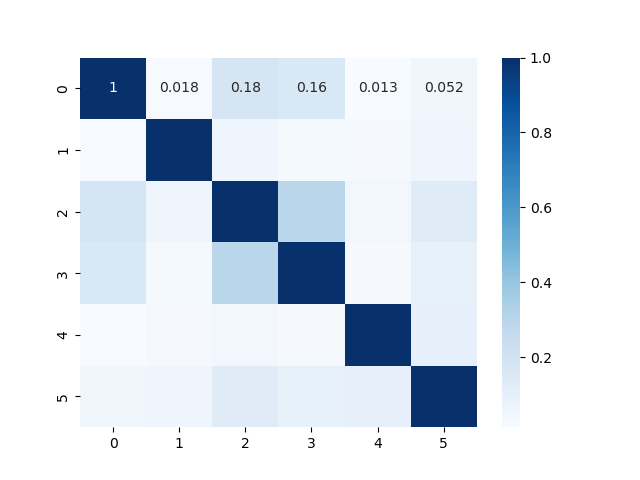
\includegraphics[width=\largeimagewidth]{images/tfidf_across_document_heatmap.png}
\caption{When all dialogue for each media is compared to each other's in aggregate, it's reassuring that the cosine similarity between any two TF-IDF vectors is extremely low.}
\end{figure}

\subsection{Classification}

A Naive Bayes Classifier was chosen because of the model's efficient training on sparse matrices, assumed independence between features, and a track record of performing well on NLP tasks^4.

After seeing the initial Naive Bayes classifier perform poorly, it became apparent that it was necessary to tune the model's hyper parameters. The following changes were made:

1. Used random over-sampling to balance the dataset, so the classifier does not bias against an under-represented media or speaker in the corpus.

2. Extended the n-gram range from one to three to capture short expressions and catch-phrases in addition to individual words.

3. Lowered the maximum document frequency from 1 to 0.99, removing the noise of any word or phrase that is present in every speaker's dialogue.

The final model:

\begin{verbatim}
model = make_pipeline(
    TfidfVectorizer(ngram_range=(1, 3), max_df=0.99),
    SMOTE(),
    MultinomialNB()
)
\end{verbatim}

\section{Results}

\subsection{Classifying Dialogue}

Model performance was evaluated by taking the average prediction rate across all speakers or media. This was to penalize any model that classified one show or speaker at a very high rate at the cost of classifying other categories at a low rate.

\subsubsection{Within Media}
\subsubsection{Across Media}

\subsection{Assessing Speaker Variability}
While building a classifier to predict the speaker of a line of dialogue is the technical culmination of this project, it's only auxiliary for addressing the original motivation of measuring speaker distinctness.

Returning to the results of taking the top principal components from each speaker's TF-IDF matrix (Figure 6), we can glean a number of observations that we might pass on to a head writer.

\begin{enumerate}
\item Characters in \textit{Friends} use highly similar vocabulary. The show might be more endearing if more terms specific to each character were common.
\item Characters in \textit{The Simpsons} have distinct vocabulary, but clusters emerge around gender lines–Bart and Homer are close together, as are Lisa and Marge. 
\end{enumerate}


\section{Conclusion}
This is the conclusion section.

\section{Future Work}
\subsection{Model Improvements}

\begin{enumerate}
\item Add dimensionality reduction to the model to see if categorization based the top N components improves classification rate.
\item During data pre-processing, add additional speaker-level features such as role (gender, role, education level) and see how well the classifier performs at identifying these broader categories instead of the actual speaker.
\item Use different statistical models as classifiers that are well-suited for prediction of a categorical variable (Support Vector Machines, Logistic Regression, Random Forest, etc.) and compare to the performance of the Naive Bayes Model.
\item During data pre-processing, add additional speaker-level features such as role (gender, role, education level) and see how well the classifier performs at identifying these broader categories instead of the actual speaker.
\item Add stylometry as an additional model, making the model's final prediction the response with the highest weighted average between the existing model and the stylometry one. For example, it's possible that the KDE is better at predicting the subset of dialogue lines that contain long sentences and/or words, where vocabulary is better at classifying dialogue with stylometric features in the center of the distribution.
\end{enumerate}

\subsection{Model Applications}

\begin{enumerate}
\item Improve the interpretability of the clustering by exposing which vocabulary words contribute to the proximity between two speakers. Which terms do Summer and Beth share that Morty and Jerry do not? The availability of this list would expose an unconscious use of gendered language for the show writers to address.
\item Retrieve which words are commonly used by all the characters in a single piece of media but have a low presence in English overall by comparing to the word's frequency distribution in a larger English corpus. This would reveal whether the writer's quirks of vocabulary are seeping into their writing without taking the opportunity to more realistically attribute that quirk to a single character's speech.
\item Expand the dataset so that any piece of media can be compared to a benchmark for its type. While Figure 6 implies that everyone in \textit{Friends} talks the same, it's possible that \textit{Friends} actually has a more diverse speaker vocabulary than most other American sitcoms. The inverse may also be true, that while the characters in \textit{Pride and Prejudice} are dispersed on the chart, they may pale in comparison to other great works of literature like \textit{Anna Karenina} or \textit{A Tale of Two Cities}.
\end{enumerate}

\begin{enumerate}

\end{enumerate}

\section{Appendix}
\subsubsection{Select Code Sections}

\begin{enumerate}
\item \textbf{Data Preparation}: \url{github.com/wluna01/isye-6740-project/blob/main/code/data_prep.py}
\item \textbf{Data Set}: \url{github.com/wluna01/isye-6740-project/blob/main/data/dialogue.csv}
\item \textbf{Heuristics}: \url{github.com/wluna01/isye-6740-project/blob/main/code/heuristics.py}
\item \textbf{Stylometry Feature Extraction}: \url{github.com/wluna01/isye-6740-project/blob/main/code/data_feature_extraction.py}
\item \textbf{Stylometry Classifier}: \url{github.com/wluna01/isye-6740-project/blob/main/code/stylometry_classifier.py}
\item \textbf{TF-IDF Scatter Plot} \url{github.com/wluna01/isye-6740-project/blob/main/code/tf_idf_across_media.py}
\item \textbf{Naive Bayes Classifier}:: \url{github.com/wluna01/isye-6740-project/blob/main/code/nb_classifier_within_media.py}
\end{enumerate}

\subsubsection{References}

\begin{enumerate}
\item \url{direct.mit.edu/coli/article/41/3/481/1519/Computational-Constancy-Measures-of-Texts-Yule-s-K}
\item \url{statology.org/simpsons-diversity-index/}
\item \url{jstor.org/stable/30204514}
\item \url{web.archive.org/web/20180604105217id_/http://onlinepresent.org/proceedings/vol111_2015/50.pdf}
\end{enumerate}

\end{titlepage}
\end{document}
